\documentclass[
    parskip=half,
    bibliography=totoc,     % Literatur im Inhaltsverzeichnis
    captions=tableheading,  % Tabellen�berschriften
    titlepage=firstiscover, % Titelseite ist Deckblatt
    ]{scrartcl}
    
\usepackage[top=2cm, bottom=4cm, left=2cm, right=2cm]{geometry}
\usepackage{color}
\usepackage[usenames,dvipsnames]{xcolor}
\definecolor{light-red}{HTML}{FFBABA}

% LaTeX2e korrigieren.
\usepackage{fixltx2e}

% Warnung, falls nochmal kompiliert werden muss
\usepackage[aux]{rerunfilecheck}

% Deutsche Spracheinstellungen
\usepackage{polyglossia}
\setmainlanguage{german}

% Unverzichtbare Mathe-Befehle
\usepackage{amsmath}

% Viele Mathe-Symbole
\usepackage{amssymb}

% Erweiterungen f�r amsmath
\usepackage{mathtools}

% Fonteinstellungen
\usepackage{fontspec}
\defaultfontfeatures{Ligatures=TeX}

\usepackage[
    math-style=ISO,    % \
    bold-style=ISO,    % |
    sans-style=italic, % | ISO-Standard folgen
    nabla=upright,     % |
    partial=upright,   % /
    ]{unicode-math}

\setmathfont{Latin Modern Math}
\setmathfont[range={\mathscr, \mathbfscr}]{XITS Math}
\setmathfont[range=\coloneq]{XITS Math}
\setmathfont[range=\propto]{XITS Math}

% Das hquer-Symbol versch�nern
\let\hbar\relax
\DeclareMathSymbol{\hbar}{\mathord}{AMSb}{"7E}
\DeclareMathSymbol{?}{\mathord}{AMSb}{"7E}

% Richtige Anf�hrungszeichen
\usepackage[autostyle]{csquotes}

% Zahlen und Einheiten
\usepackage[
  locale=DE,                   % Deutsche Einstellungen
  separate-uncertainty=true,   % Immer Fehler mit \pm
  per-mode=symbol-or-fraction, % m/s im Text, sonst Br�che
]{siunitx}

% Chemische Formeln
\usepackage[version=3]{mhchem}

% Sch�ne Br�che im Text
\usepackage{xfrac}

% Floats innerhalb einer Section halten
\usepackage[section, below]{placeins}

% Captions sch�ner machen.
\usepackage[
    labelfont=bf,        % Tabelle x: Abbildung y: ist jetzt fett
    font=small,          % Schrift etwas kleiner als Dokument
    width=0.9\textwidth, % Maximale Breite einer Caption schmaler
    ]{caption}

% Subfigure, subtable, subref
\usepackage{subcaption}

% Grafiken einbinden
\usepackage{graphicx}

% Gr��ere Variation von Dateinamen m�glich
\usepackage{grffile}

% Standardplatzierung f�r Floats einstellen
\usepackage{float}
\floatplacement{figure}{htbp}
\floatplacement{table}{htbp}

% Sch�ne Tabellen
\usepackage{booktabs}

% Seite drehen f�r breite Tabellen
\usepackage{pdflscape}

% Literaturverzeichnis
\usepackage{biblatex}

% Quellendatenbank
\addbibresource{lit.bib}
\addbibresource{programme.bib}

% Hyperlinks im Dokument
\usepackage[
    unicode,
    pdfusetitle,    % Titel, Autoren und Datum als PDF-Attribute
    pdfcreator={},  % PDF-Attribute s�ubern
    pdfproducer={}, % "
    ]{hyperref}
    
% Erweiterte Bookmarks im PDF
\usepackage{bookmark}

% Trennung von W�rtern mit Strichen
\usepackage[shortcuts]{extdash}

% Blindtext erzeugen
\usepackage{blindtext}

% Support f�r mdframed
\usepackage{kvoptions}
\usepackage{xparse}
\usepackage{etoolbox}
\usepackage{tikz}

% Sch�ne mehrseitige Rahmen um Text erzeugen
\usepackage{mdframed}
\mdfsetup{skipabove=\topskip,skipbelow=\topskip}
% Neue Mathematikbefehle
\DeclareMathOperator{\rank}{rang}
\DeclareMathOperator{\cond}{cond}
\newcommand{\up}{\mathup}
\newcommand{\R}{\mathbb{R}}
\newcommand{\N}{\mathbb{N}}
\newcommand{\upD}{\mathup{\Delta}}

% Wichtiger Befehl zur Erstellung einer blauen Box um einen Text
\newcommand\mybox[2][]{\tikz[overlay]\node[fill=blue!20,inner sep=4pt, anchor=text, rectangle, rounded corners=1mm,#1] {#2};\phantom{#2}}
\newenvironment{Versuch}[1]{
    \mdfsetup{
        innertopmargin=8pt,
        linecolor=blue!20,
        linewidth=2pt,
        topline=true,
        backgroundcolor=blue!20
        }
    \begin{mdframed}
    \Large{\textbf{#1}}
    \end{mdframed}}
    {}

\newenvironment{Stichworte}{
    \mdfsetup{
        frametitle={\mybox[fill=blue!20]{\Large{Stichworte}}},
        frametitleaboveskip=0pt,
        innertopmargin=10pt,
        linecolor=blue!20,
        linewidth=2pt,
        topline=true,
        backgroundcolor=white
        }
    \begin{mdframed}}
    {\end{mdframed}}    
    
\newenvironment{Zielsetzung}{
    \mdfsetup{
        frametitle={\mybox[fill=blue!20]{\Large{Zielsetzung}}},
        frametitleaboveskip=0pt,
        innertopmargin=10pt,
        linecolor=blue!20,
        linewidth=2pt,
        topline=true,
        backgroundcolor=white
        }
    \begin{mdframed}}
    {\end{mdframed}}

\newenvironment{Theorie}{
    \mdfsetup{
        frametitle={\mybox[fill=blue!20]{\Large{Theorie}}},
        frametitleaboveskip=0pt,
        innertopmargin=10pt,
        linecolor=blue!20,
        linewidth=2pt,
        topline=true,
        backgroundcolor=white
        }
    \begin{mdframed}}
    {\end{mdframed}}

\newenvironment{Durchführung}{
    \mdfsetup{
        frametitle={\mybox[fill=blue!20]{\Large{Durchführung}}},
        frametitleaboveskip=0pt,
        innertopmargin=10pt,
        linecolor=blue!20,
        linewidth=2pt,
        topline=true,
        backgroundcolor=white
        }
    \begin{mdframed}}
    {\end{mdframed}}
    
\newenvironment{Auswertung}{
    \mdfsetup{
        frametitle={\mybox[fill=blue!20]{\Large{Auswertung}}},
        frametitleaboveskip=0pt,
        innertopmargin=10pt,
        linecolor=blue!20,
        linewidth=2pt,
        topline=true,
        backgroundcolor=white
        }
    \begin{mdframed}}
    {\end{mdframed}}
    
\newenvironment{Diskussion}{
    \mdfsetup{
        frametitle={\mybox[fill=blue!20]{\Large{Diskussion}}},
        frametitleaboveskip=0pt,
        innertopmargin=10pt,
        linecolor=blue!20,
        linewidth=2pt,
        topline=true,
        backgroundcolor=white
        }
    \begin{mdframed}}
    {\end{mdframed}}

\newenvironment{Merke}{
    \mdfsetup{
        frametitle={\mybox[fill=red]{\Large{Merke}}},
        frametitleaboveskip=0pt,
        innertopmargin=5pt,
        linecolor=red,
        linewidth=1pt,
        topline=true,
        backgroundcolor=light-red
        }
    \begin{mdframed}}
    {\end{mdframed}}

\newenvironment{Appendix}{
    \mdfsetup{
        frametitle={\mybox[fill=blue!20]{\Large{Appendix}}},
        frametitleaboveskip=0pt,
        innertopmargin=10pt,
        linecolor=blue!20,
        linewidth=0pt,
        topline=false,
        backgroundcolor=white
        }
    \begin{mdframed}}
    {\end{mdframed}}
    
\begin{document}

    \begin{Versuch}{V354: Gedämpfte und erzwungene Schwingungen}
	\begin{Stichworte}
		Analogie: Schwingfähige Systeme in Mechanik und Elektrik.

		Komplexe Amplitude,
		Phasenwinkel $\phi$,
		Güte $q$,
		Resonanzbreite

	\end{Stichworte}

	\begin{Zielsetzung}
		Gedämpfte und erzwungene Schwingungen und deren Verhalten studieren. Hierfür werden elektrische Schaltungen in Analogie gebaut und Spannungen gemessen.
	\end{Zielsetzung}

    \begin{Theorie}
    	\section*{Dämpfung}
       	Anstelle von mechanischen Systemen werden elektrische Schaltungen betrachtet.
       	Mit einem Serienschwingkreis, bestehend aus Widerstand $R$, Kondensator $C$ und Spule $L$, wird ein gedämpftes System simuliert.
       	\begin{equation}
			U_\text{R}(t)+U_\text{C}(t)-U_\text{L}(t)=0
			\label{systemgleichung}
		\end{equation}
		\begin{equation}
			U_\text{R}(t) = R\cdot I(t)\qquad
			U_\text{C}(t) = \frac{Q(t)}{C}\qquad
			U_\text{L}(t) = -L\frac{\mathup{d}I(t)}{\mathup{d}t},
		\label{eq:austauscher}
		\end{equation}
		Es gilt die Systemgleichung 
		\begin{equation}
			\frac{\mathup{d^2}I(t)}{\mathup{d}t^2}+\frac{{R}}{{L}}\frac{\mathup{d}I(t)}{\mathup{d}t}+\frac{1}{{LC}}I(t)=0,
		\end{equation}
		ihre allgmeinen Lösung
		\begin{equation}
			I(t) = A_1\cdot e^{{\omega_1}t} +A_2\cdot e^{{\omega_2}t}
			\label{eq:allgloesung}
		\end{equation}
		mit der Abkürzung
		\begin{equation}
			{\omega_{1,2}}= -\frac{{R}}{2{L}}\pm\sqrt{\underbrace{\frac{{R^2}}{4{L^2}}-\frac{1}{{LC}}}_{\text{Diskriminante}}}.
			\label{eq:allomega}
		\end{equation}
		Durch die Diskriminante sind folgende Fälle bestimmbar
		\begin{description}
			\item [Schwingfall] \begin{equation}
									I(t) = e^{-\frac{{R}}{2{L}}\,t}\Bigl(A_1 \sin\Bigl(\sqrt{\frac{1}{{LC}}-\frac{{R^2}}{4{L^2}}}\, t\Bigr)+A_2 \cos\Bigl(\sqrt{\frac{1}{{LC}}-\frac{{R^2}}{4{L^2}}}\,t\Bigr)\Bigr).
								\end{equation}
			\item [ap. Grenzfall] \begin{equation}
									I(t) = A_1 e^{-\frac{{R}}{2{L}}\,t}+A_2 t e^{-\frac{{R}}{2{L}}\,t}.
								  \end{equation}
			\item [Kriechfall] \begin{equation}
									I(t)= A_1 e^{\omega_1 t} + A_2 e^{\omega_2 t}.
								 \end{equation}
		\end{description}
		Für die Schwingperiode gilt die Thomsonsche Schwingungsgleichung und die Abklingdauer
		\begin{equation}
			T_0 = \frac{2π}{{ω_0}} = \mathup{2π} \sqrt{LC}\,;\qquad T_\text{ex} = \frac{{2L}}{{R}}.
			\label{eq:thomson}
		\end{equation} 
	
		\section*{Zwang}
		Betrachtet wird die am Kondensator anliegende Spannung $U_\text{C}$.
		Zusätzlich zur Systemgleichung \eqref{systemgleichung} kommt die äußere Zwangsspannung $U_\text{Zwang}(t)$
		\begin{equation}
				{LC}\frac{{d^2}U_\text{C}}{{d}t^2} +{RC}\frac{{d}U_\text{C}}{{d}t} +U_\text{C}=U_\text{Zwang}(t)=U_0\cdot\exp{i\omega t}.
				\label{eq:DGLerzw}
		\end{equation}
		Die Lösung setzt sich aus homogener und inhomogener Lösung zusammen, die homogene Lösung klingt in kurzer Zeit ab und wird vernachlässigt.
		Bei dem nun gewählten \emph{komplexe Amplitude}-Ansatz  $U_{C}(\omega,t)= \tilde{U}_{\omega}(\omega)\cdot e^{i\omega t}$,
		$\tilde{U}_{\omega}(\omega)\in\mathbb{C}$, 
		ist der Phasenwinkel $\mathup{arg}(\tilde{U}_{\omega})=\phi$ und Betrag $|\tilde{U}_{\omega}|\in\R$.
		Dies führt nach Einsatz und Kürzen der Exponentialfunktion zu
		\begin{equation}
			U_0 = - {LC}\omega^2 \tilde{U}_\mathup{\omega}(\omega) + i\omega{RC}\tilde{U}_\mathup{\omega}(\omega) + \tilde{U}_\mathup{\omega}(\omega).
		\end{equation}
		und damit schließlich zu
		\begin{subequations}
			\begin{equation}
				|\tilde{U}_{\omega}(\omega)|= \frac{U_0}{\Bigl(\sqrt{(1 − {LC}\omega^2)^2 +ω^2{R^2C^2}}\Bigr)}
				\label{eq:yes}
			\end{equation}
			\begin{equation}
				\mathup{tan}(\phi) = \frac{\mathup{Im}(\tilde{U}_{\omega})}{\mathup{Re}(\tilde{U}_{\omega})}=\frac{ω{RC}}{{LC}ω^2-1}
			\end{equation}
		\end{subequations}

		Sonderfälle:
		\begin{equation}
		 	\lim_{\omega\to\infty} \tilde{U}_\mathup{\omega} =0, \qquad \lim_{\omega\to 0}\tilde{U}_\mathup{\omega} = U_0
		\end{equation}
		auf.

		Es existiert eine Resonanzfrequenz $\mathup{\omega_0} = \sqrt{\frac{1}{{LC}}-\frac{{R^2}}{4{L^2}}}$, die durch Dämpfung und Eigenfrequenz gegeben ist.
		Sie ist die neue Schwingfrequenz des Systems.
		Bei Erregung des Systems mit $\omega \approx \mathup{\omega_0}$ kommt es zur Resonanz; 
		das System schwingt mit einer Spannungsamplitude $U_\text{C,max}$ größer als die Erregeramplitude $U_0$,
		\begin{equation}
			U_\text{C,max}= \underbrace{\frac{1}{\mathup{\omega_0}RC}}_{\text{Güte}\, q} U_0. 
			\label{eq:maxspannung}
		\end{equation}

		Zur Charakterisierung des \emph{Resonanzverhaltens} 
		(nur im Schwingfall) werden die Grenzwerte
		$\mathup{\omega_\pm}$ betrachtet, 
		bei welchen die Spannung $U_\mathup{C}$ auf den 
		$\sfrac{1}{\sqrt{2}}$-Teil des Maximalwertes $U_\mathup{C,max}$ abfallen.  
		Für die so beschriebene \emph{Resonanzbreite} gilt
		\begin{equation}
			\mathup{2\pi\Delta}\, f = \mathup{ω_+} − \mathup{ω_−} \approx \frac{{R}}{{L}}.
			\label{eq:deltaf}
		\end{equation}
		Ausgehend von der  Erregerspannung $U_0$ fällt der Betrag der Spannung $U_\mathup{C}$  mit $\frac{1}{\omega^2}$ ab.

		Der \emph{Phasenwinkel $\phi$} zwischen der Kondensatorspannung $U_\mathup{C}(t)$ und der Erregerspannung $U(t)$.\\
		Für die Frequenz $\omega^2 = \frac{1}{{LC}}$ besteht zwischen der Kondensatorspannung $U_\text{C}$ und der Erregerspannung $U$ ein Winkel von $\phi =-\frac{\pi}{2}$.
		Für große Frequenzen nähert sich die Phasenwinkel $\phi$ dem stationären Wert $\pi$ an.

	\end{Theorie}
    
    \begin{Durchführung}
        Es wird auf einem Oszilloskop die am Kondensator anliegende Spannung angezeigt.

        \emph{Dämpfung}:
        Es wird an den Kondensator ein Generator angeschlossen, der mit einer so geringer Frequenz eine Rechteckspannung liefert, dass der Schwingkreis frei schwingen kann.
       
        \emph{Zwang}:
        Es wird an den Kondensator ein Generator für vers. Frequenzen angeschlossen.
        Gemessen wird die Abhängigkeit der Kondensatorspannung $U_\text{C}(t)$ und des Phasenwinkels $\phi$ von der Frequenz der Erregerspannung.
        Hierzu wird mit einer Reihe von vers. Generatorfrequenzen der Betrag $U_\text{C}(t)$ direkt gemessen und der Phasenwinkel $\phi$ durch den Zeitversatz der Nulldurchgänge von Generator und Kondensator bestimmt.
    \end{Durchführung}        
    
    \begin{Auswertung}
    	\begin{itemize}
    		\item Im Fall der gedämpften Schwingung fällt die Amplitude (sehr genau) exponentiell mit der Zeit ab.
    		\item Der ap. Grenzfall lässt sich durch Bisektion finden.
    		\item Die Bilder für Schwingfall, ap. Grenzfall und Kriechfall sind im Appendix zu finden.
    		\item Die experimentell ermittelten Widerstände sind geringer als die theoretisch benötigten Werte.

    		\item Die \emph{Resonanzkurve} ist im Appendix zu finden.
    		\item Die \emph{Versatzkurve} ist im Appendix zu finden.

    	\end{itemize}
    \end{Auswertung}

    \begin{Diskussion}
    	\begin{itemize}
    		\item Große Messunsicherheiten: viele, fehlerbehafteten Größen
    		\item Analogie zwischen Mechanik und Elektrik ist sicher.
    	\end{itemize}
    \end{Diskussion}

    \begin{Merke}
    	Unbedingt die Resonanz- und Versatzkurve einprägen.
    \end{Merke}

\newpage
\thispagestyle{empty}
    \begin{Appendix}
    		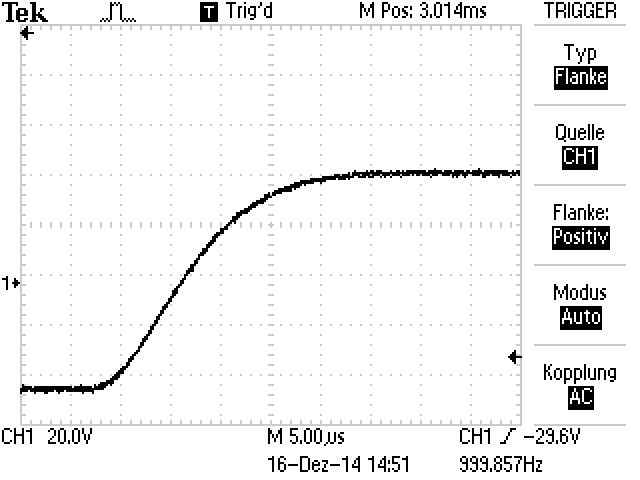
\includegraphics[width=0.3\textwidth]{build/Bilder/kr.JPG}
    		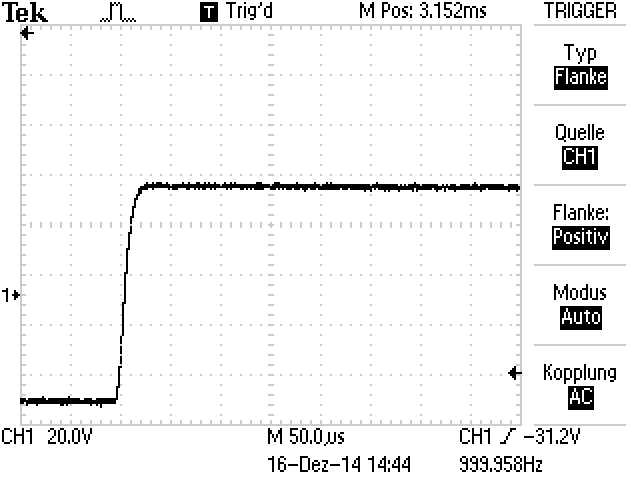
\includegraphics[width=0.3\textwidth]{build/Bilder/ap.JPG}
    		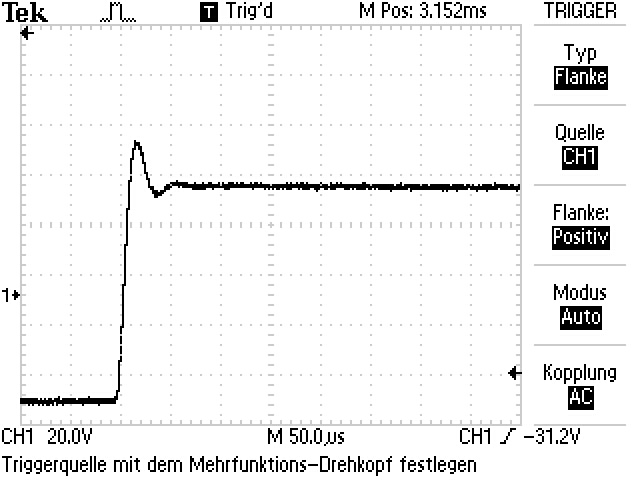
\includegraphics[width=0.3\textwidth]{build/Bilder/sw.JPG}

    		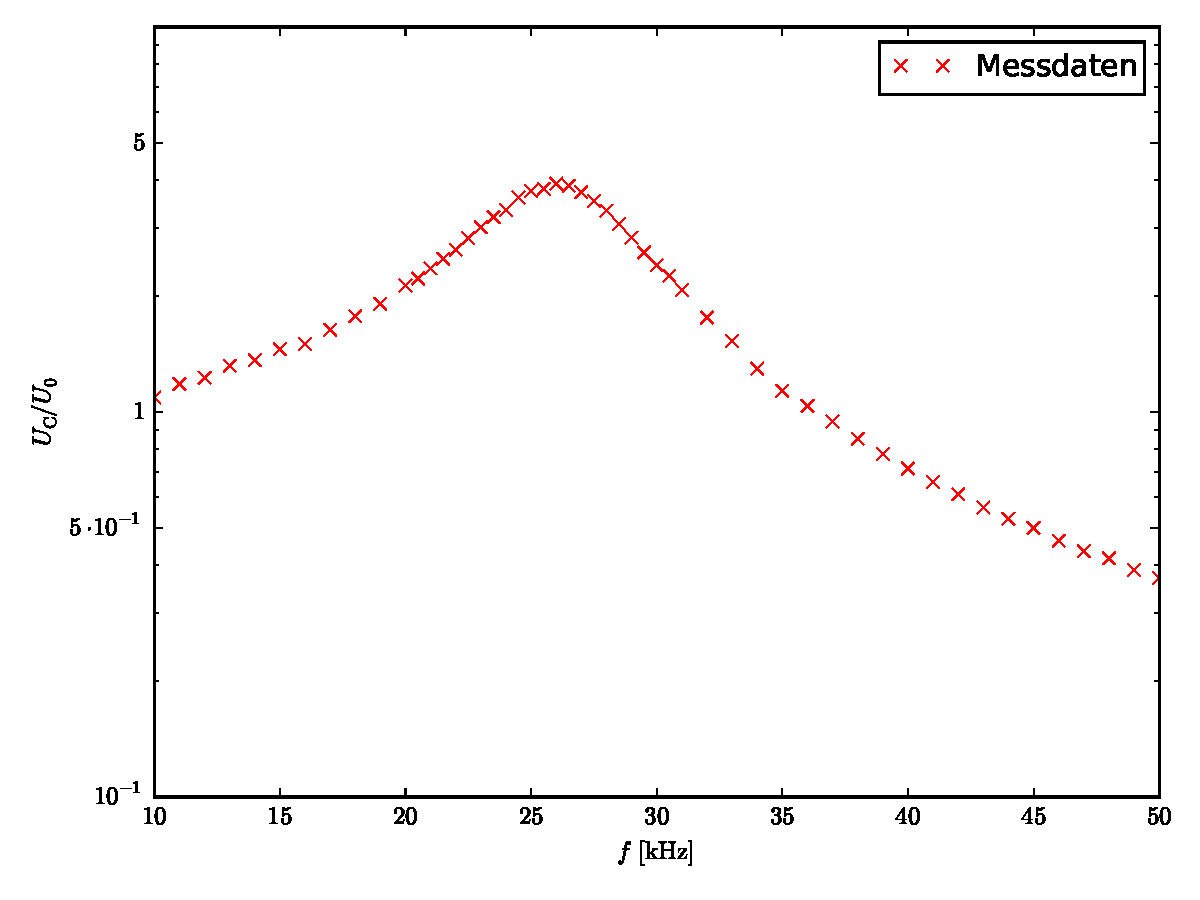
\includegraphics[width=0.3\textwidth]{build/Bilder/rk.pdf}
    		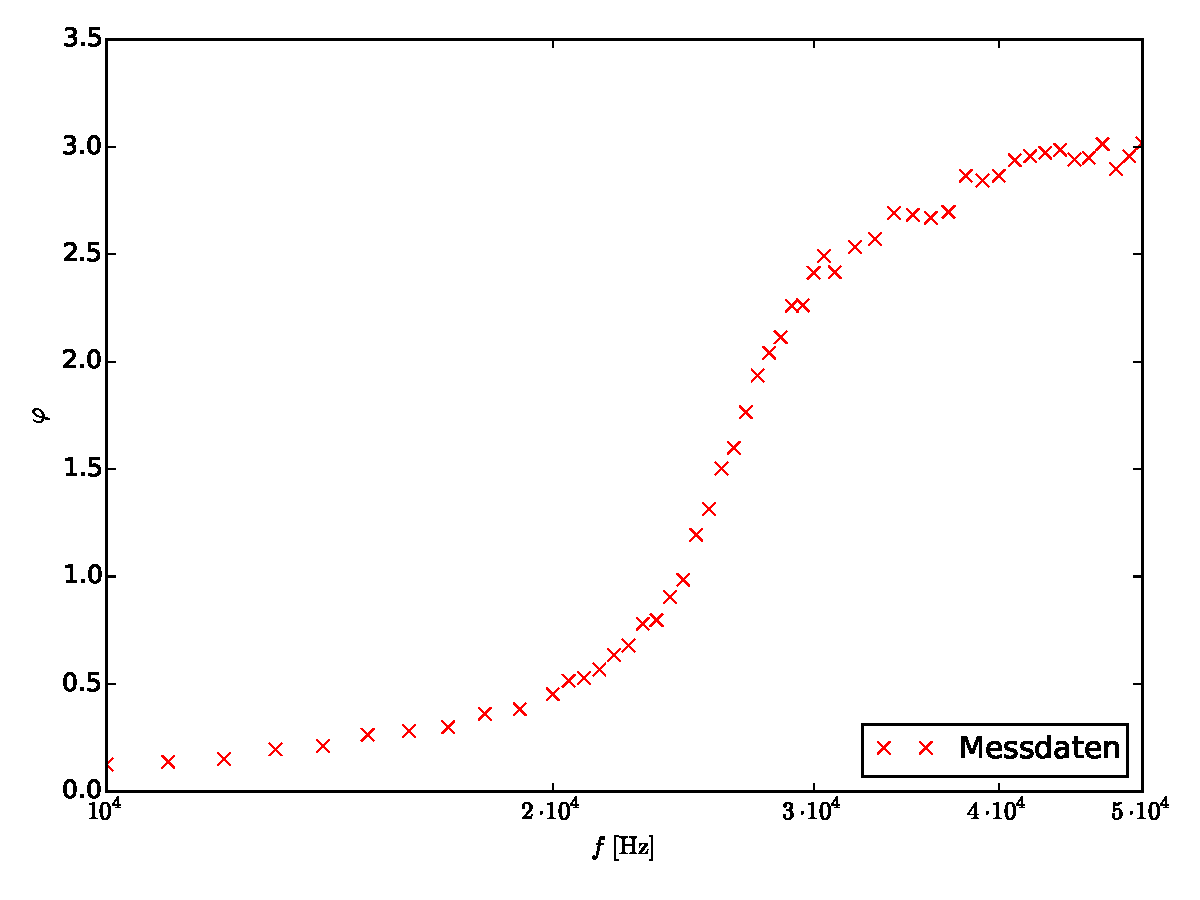
\includegraphics[width=0.3\textwidth]{build/Bilder/vk.pdf}
    		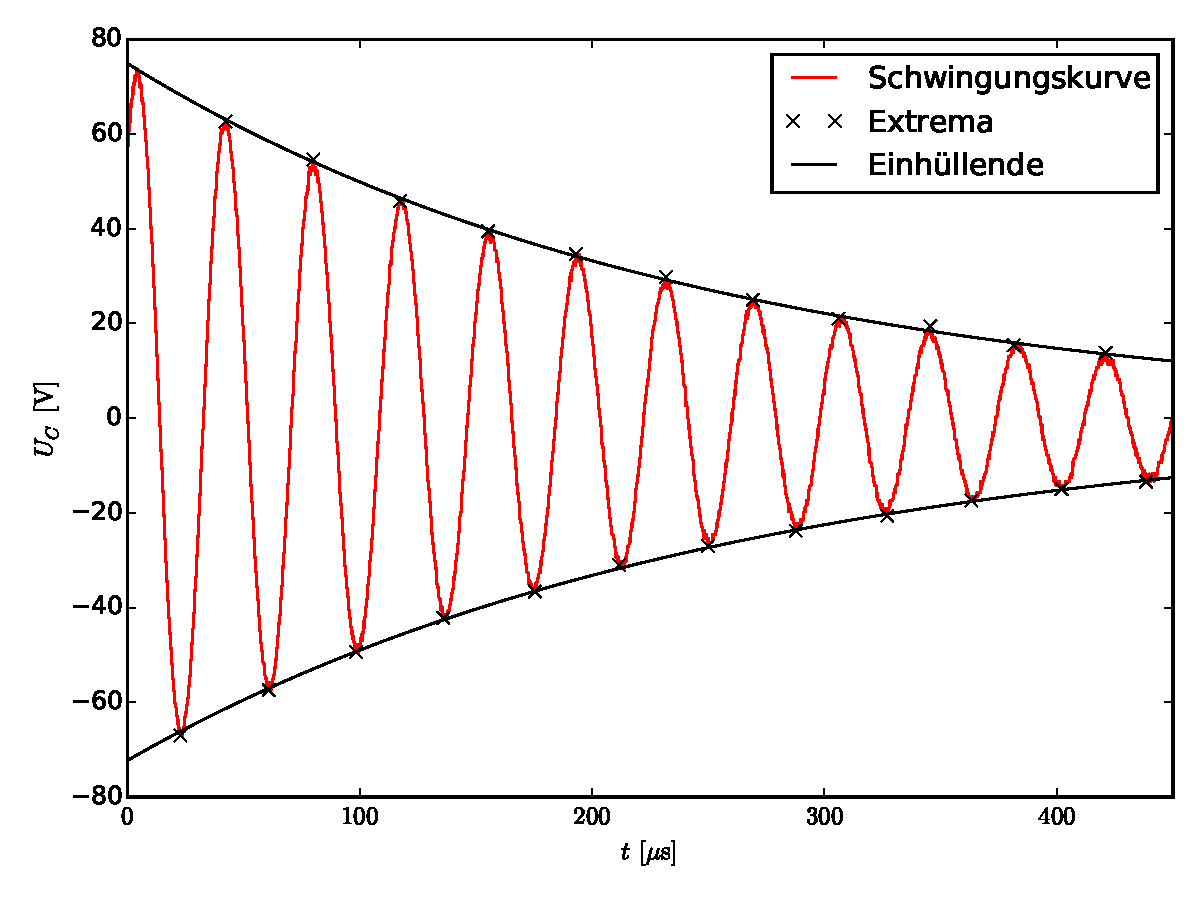
\includegraphics[width=0.3\textwidth]{build/Bilder/ak.pdf}
    \end{Appendix}
    \end{Versuch}
\end{document}